\documentclass[11pt]{article}

\usepackage{xltxtra}
\usepackage{fontspec}
\setmainfont{TeX Gyre Pagella}

\usepackage[a4paper, top=2cm, bottom=2cm, left=3cm, right=3cm]{geometry}

\usepackage{amsmath}
\usepackage{graphicx}
\usepackage{hyperref}
\usepackage{verbatim}
\usepackage{paralist}
\usepackage{minted}

\usepackage[normalem]{ulem}

% macro for MetaModelElements
\newcommand{\smme}[1]{\uline{\texttt{#1}}}
\newcommand{\tmme}[1]{\texttt{#1}}

\newcommand{\email}[1]{\href{mailto:#1}{\texttt{#1}}}
\newcommand{\myemail}[0]{\email{horn@uni-koblenz.de}}

%% Schusterjungen und Hurenkinder verhindern. Das sind einzelne Zeilen von
%% Absätzen am Anfang oder Ende einer Seite.
\clubpenalty = 10000
\widowpenalty = 10000
\displaywidowpenalty = 10000


\title{The TTC 2013 Flowgraphs Case}
\author{Dipl.-Inform. Tassilo Horn\\
  \myemail\\
  \vspace{0.3cm}\\
  University Koblenz-Landau, Campus Koblenz\\
  Institute for Software Technology\\
  Universitätsstraße 1, 56070 Koblenz, Germany}

\begin{document}

\maketitle

\begin{abstract}
  This case for the Transformation Tool Contest 2013 is about evaluating the
  flexibility of transformation languages and tools.  It consists of four tasks
  requiring different capabilities.  Two tasks deal with typical model-to-model
  transformation problems, there's a model-to-text problem, there are two
  in-place transformation problems, and finally there's a task dealing with
  validation of models resulting from the transformations.

  The tasks build upon each other, but the transformation case project also
  provides all intermediate models, thus making it possible to skip tasks that
  are not suited for a particular tool.

  All models and metamodels are provided in the EMF/Ecore format.  However,
  user's of other modeling frameworks are also encouraged to participate.
\end{abstract}

\sloppy

\section{Objective of the Case}
\label{sec:objective}

The objective of this case is to allow participants to demonstrate their
transformation tool's flexibility.  Therefore, the different tasks require
several different transformation capabilities.

Task 1 deals with a typical model-to-model transformation problem.  Given an
abstract syntax graph of a Java program comforming to the very detailed EMFText
JaMoPP metamodel \cite{jamopp09}, a new model, the structure graph of the
original program, conforming to a much more abstract and simple metamodel has
to be generated.  Embedded in this task is a model-to-text transformation.  In
the JaMoPP model, a simple statement like \verb|int i = a + b;| is expressed as
a whole bunch of interrelated objects.  In the target model, we only want one
single \verb|SimpleStmt|, but its \verb|txt| attribute should be set to the
original Java syntax: \verb|int i = a + b;|.

In task 2, the structure graph resulting from task 1 should be enhanced with
control flow information, i.e., every statement or expression has to be
connected with its possible successors as defined by the Java semantics
\cite{Java7Spec}.  This is an in-place transformation task that's suited for
graph transformation tools but can also be tackled algorithmically.

Task 3 is similar to task 2 from a technical point of view, that is, it is also
an in-place transformation.  Based on the control flow graph resulting from
task 2, data flow information has to be synthesized.  This also requires some
additions to the model-to-model transformation from task 1.  Again, this task
is suited to be tackled with graph transformations or algorithmically.

The context of task 4 is a bit offside the strict transformation context.
Nevertheless, it tackles the important challenge of model validation.  Given
the fact that you as transformation engineer put all your efforts in the
transformation tasks, can you offload testing to developers that have a good
Java knowledge but know nothing about MDE, EMF, or whatever modeling technology
you are using?

Because every task builds upon the results of previous tasks, the intermediate
models are also provided to allow participants to defer or skip tasks not
particulary suited for their tools, or to allow teams for developing solutions
in parallel.  For this reason, there are also no \emph{core} and
\emph{extension} tasks.  To participate, only one arbitrary task has to be
solved, but of course scoring high presumably requires solving more tasks.


All models and metamodels are provided in the EMF/Ecore format.  However,
user's of other modeling frameworks are also encouraged to participate.  If
requested, the case proponent is willing to help writing an export tool to
other formats such as GXL \cite{GXL02}.


\section{Detailed Task Description}
\label{sec:task-descr}

\paragraph{Structure of the Case Project.}

The case project is available on GitHub\footnote{This case's project:
  \url{https://github.com/tsdh/ttc-2013-flowgraphs-case}}. The top-level folder
\verb|ttc-2013-flowgraphs-case| contains several directories.  The directory
\verb|desc| contains the case description your are reading right now.

The \verb|metamodel| directory contains the target metamodel as Ecore file
(\verb|FlowGraph.ecore|) including PDF images with several views of it focusing
on the specific tasks.  \verb|StructureGraph.pdf| shows the target metamodel of
task 1, \verb|ControlFlowGraph.pdf| shows the metamodel classes important for
task 2, and \verb|DataFlowGraph.pdf| shows the metamodel classes important for
task 3.

The \verb|src| folder contains several Java classes.  Every class contains just
one single method.  For every class, one model will be generated as source for
task 1.  If you need more models to test your transformations, simply put a new
Java file in this directory.

The \verb|jamopp| directory contains the JaMoPP-Parser as JAR file that
generates EMF models conforming to the JaMoPP metamodel out of Java source code
files.

Initially, the \verb|models| directory is empty.  Top-level, there're scripts
\verb|gen-models-from-src.sh| (for Unices) and \verb|gen-models-from-src.bat|
(for Windows).  When being run, they use JaMoPP to parse all Java files in
\verb|src| and create corresponding models (file extension \verb|java.xmi|) in
\verb|models|.  Those are valid source models for task 1.  Additionally, the
JaMoPP parser also serializes the JaMoPP metamodel next to the model files.  It
is called \verb|java.ecore|\footnote{It'll also create a file
  \texttt{layout.ecore} containing classes that can be used to annotate
  abstract syntax graphs with layout information such as indentation, but this
  is of no importance for this case.}.

The \verb|results| folder contains all intermediate and final target models
including visualizations.  You can use them to validate your own results, or
use them as source models for later tasks in case you skip an earlier task.

Finally, the \verb|evaluation| directory contains an OpenDocument spreadsheet
that will be used for scoring the solutions during the evaluation.


\subsection{Task 1: Structure Graph}
\label{sec:task1-structure-graph}

The first task requires writing a model-to-model transformation.  The source
models are the Java abstract syntax graphs conforming to the JaMoPP metamodel
that are created by the \verb$gen-models-from-src.[sh|bat]$ scripts.  The
JaMoPP metamodel covers the complete syntax of Java 7.  However, to restrict
the size of the transformation, the elements actually contained in the source
models is very limited.  For every \verb|*.java| file, the corresponding model
contains one compilation unit containing exactly one class with exactly one
method.  The method may have parameters.  In the method's body, there may be
local variable declarations, arithmetic expressions (only \verb|+|, \verb|-|,
\verb|*|, and \verb|/|), assignments, unary modification expressions
(\verb|i++;| and \verb|i--;|), \verb|return| statements, and blocks.  There may
be \verb|if|-statements and \verb|while|-loops with a boolean expression as
condition.  Statements may be labeled, and \verb|break|/\verb|continue| may be
used with or without target label.  Section~\ref{sec:list-used-jamopp} in the
appendix lists all actually used concrete JaMoPP classes.

The target metamodel of the transformation is depicted in
Figure~\ref{fig:structure-graph-mm}.

\begin{figure}[h!]
  \centering
  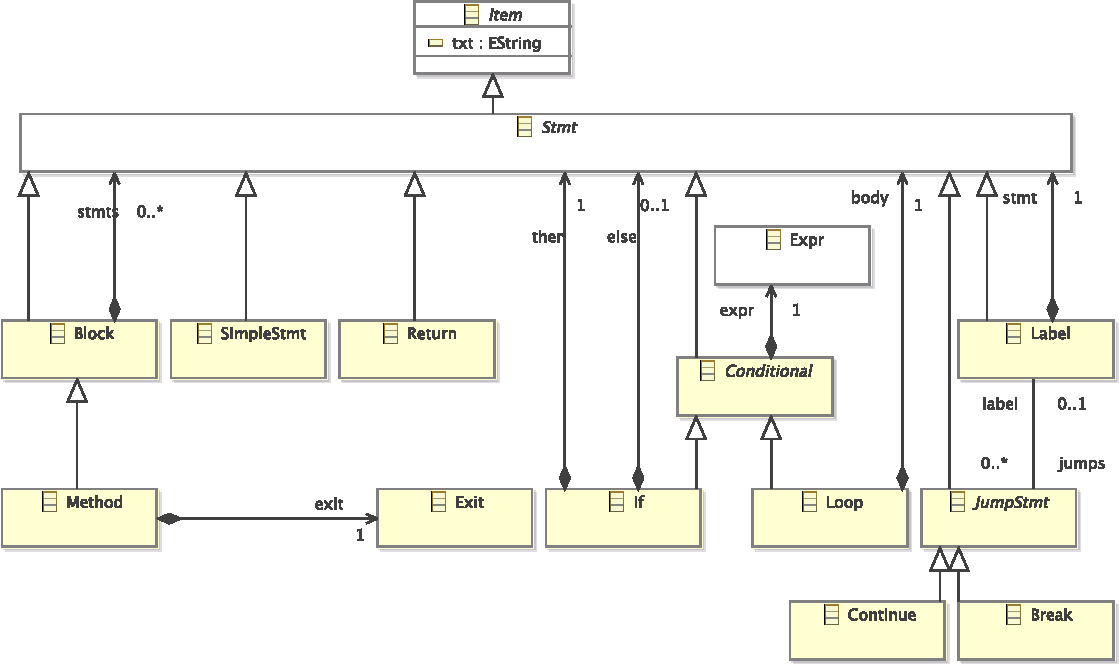
\includegraphics[width=\linewidth]{../metamodel/StructureGraph}
  \caption{The target structure graph metamodel}
  \label{fig:structure-graph-mm}
\end{figure}

The structure graph metamodel is very similar to the original JaMoPP metamodel
from a structural point of view.  The major difference is that statements and
expressions are represented as one single object instead of being split up any
further.  Another difference is that every \verb|Method| has exactly one
\verb|Exit|.  There is no correspondence in Java, but it's a synthetic element
added in favour of task 3.  No matter how a method is exited, the last object
in a method's control flow graph is the method's \verb|Exit|.

All metamodel classes extend the abstract \verb|Item| class, even the class
\verb|Expr| although not visible in Figure~\ref{fig:structure-graph-mm} because
an abstract, intermediate class between \verb|Item| and \verb|Expr| is not
displayed for readabily reasons.  \verb|Item| declares a \verb|txt| attribute.
The transformation has to set the value of this attribute to the concrete Java
syntax of the statement or expression, that is, there is a model-to-text
transformation embedded in this model-to-model transformation.  For example,
for a local variable statement with a decimal integer literal as initial value
like \verb|int i = 17;| in the JaMoPP model, a \verb|SimpleStmt| has to be
created and its \verb|txt| attribute has to be set to \verb|int i = 17;|.
Exceptions from this rule are all structured statements: the \verb|txt| value
of a \verb|Block| is always \verb|{...}|, the value for an \verb|If| is always
\verb|if|, the value for a \verb|Method| with name \verb|foo| is always
\verb|foo()| (no matter of the parameters).  The artificial \verb|Exit| objects
should have the value \verb|Exit| set.

With the exception of \verb|Break| and \verb|Continue| objects referring to
their target \verb|Label|, the structure graphs created by the transformation
are simple trees that reflect the containment relationships of the method and
its statements.

For example, Listing~\ref{lst:sg-ex} shows the method defined in
\verb|Test1.java|.

\begin{listing}
  \begin{minted}{java}
public static void testMethod(int a) {
    int i = a * 2;
    i = i + 19;
    while (i > a) {
        if (a < 1) {
            return;
        } else if (a == 1) {
            break;
        }
        i--;
    }
}
  \end{minted}
  \caption{An example Java method (\texttt{Test1.java})}
  \label{lst:sg-ex}
\end{listing}

The resulting target model is visualized in Figure~\ref{fig:sg-test1} in
Appendix~\ref{sec:result-models}.


\subsection{Task 2: Control Flow Graph}
\label{sec:task2-cf-graph}

This task deals with an in-place transformation problem.  The semantics of the
Java programming language should be integrated into the structure graphs
created by the previous transformation.  The task is to perform an
intra-procedural control flow analysis.  Any statement should be connected to
the statement that follows it in the method's control flow.

Figure~\ref{fig:control-flow-mm} shows the relevant metamodel excerpt.

\begin{figure}[h!]
  \centering
  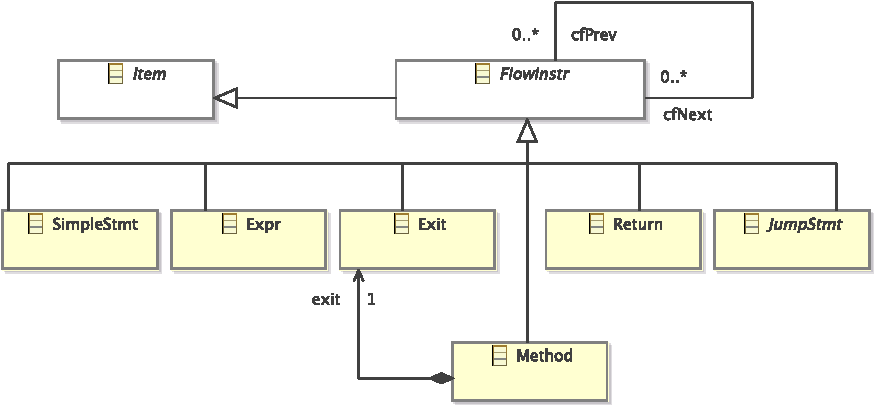
\includegraphics[width=0.8\linewidth]{../metamodel/ControlFlowGraph}
  \caption{Metamodel classes related to control flow}
  \label{fig:control-flow-mm}
\end{figure}

Simple statements, expressions, the synthetical exits, methods, \verb|return|,
and the jump statements \verb|break| and \verb|continue| extend
\verb|FlowInstr|.  Every flow instruction knows it immediate control flow
predecessors (\verb|cfPrev|) and successors (\verb|cfNext|).  It's those links
the transformation has to synthesize from the structure graph.

Blocks, labels, loops, and if-statements don't participate in the control flow.
Instead, when control flow reaches a block, the first flow instruction in the
block is the control flow successor of the previous flow instruction.

Since blocks may be nested in other blocks, the \emph{first} flow instruction
is actually the first one reachable by a depth-first search.  This \emph{first}
semantics apply to whole description of this task.

In case of a label, the first flow instruction in the statement which is
labeled is the control flow successor.

In case of loops and if-statements, the successor is their test expression.
This expression has in turn two control flow successors.  If it is a test
expression of a loop, the successors are the first flow instruction in the
loop's body, and the first flow instruction following the loop.  If it is a
test expression of an if-statements, the first successor is the first flow
instruction in then-statement.  If there is an else-statement, its first flow
instruction is the other control flow successor.  Otherwise, the other
successor is the first flow instruction in the statement following the
if-statement.

The control flow successor of a \verb|Method| is its first flow instruction,
and \verb|Return| statements always have the method's \verb|Exit| as control
flow successor.

The most complex control flow rules apply to the jump statements \verb|Break|
and \verb|Continue|.  Without a target label, the control flow successor of a
\verb|Break| is the first flow instruction in the statement following the
immediately surrounding loop, and the successor of a \verb|Continue| is the
test expression of the immediately surrounding loop.  With a target label
\verb|x|, the control flow successor of a \verb|Break| is the first flow
instruction in the statement after the statement labeled \verb|x|, and the
successor of a \verb|Continue| is the the expression of the surrounding loop
labeled \verb|x|\footnote{Interestingly, using \texttt{break x;} it is possible
  to jump out of a block labeled \texttt{x}, i.e., in contrast to
  \texttt{continue}, the labeled statement doesn't need to be a loop.}.

The method in Listing~\ref{lst:java-ex-cf} is the method defined in
\verb|Test2.java|.

\begin{listing}
  \begin{minted}{java}
public static void testMethod(int a) {
    int i = a * 2;
    while (i > a) {
        if (a < 1) {
            return;
        } else if (a == 0) {
            continue;
        }
        i++;
    }
}
  \end{minted}
  \caption{An example Java method with complex control flow
    (\texttt{Test2.java})}
  \label{lst:java-ex-cf}
\end{listing}

It's structure graph that is the result of task 1's transformation is the input
to the control flow transformation.  The result control flow model is
visualized in Figure~\ref{fig:cfg-test2} in Appendix~\ref{sec:result-models}.
In case you haven't tackled task 1 yet, it is also included in this project as
\verb|results/Test2-StructureGraph.xmi|.  The control flow transformation
should create a model equivalent to \verb|results/Test2-ControlFlowGraph.xmi|.


\subsection{Task 3: Data Flow Graph}
\label{sec:task3-df-graph}

In this task, an intra-procedural data flow analysis should be performed.  This
can be done based on the control flow graph, but currently, one important piece
of information is missing from it: for every flow instruction, we need to know
which variables it reads and writes.  Therefore, this task is twofold:

\begin{compactenum}
\item Enhance the model-to-model transformation from task 1 so that it also
  creates \verb|Var| objects for local variables and \verb|Param| objects for
  method parameters, and connect each flow instruction to the variables it
  reads and writes.
\item Write a data flow transformation taking the control flow graph resulting
  from applying task 2's transformation on the result of the enhanced
  java-to-structure-graph transformation, that synthesizes data flow links.
\end{compactenum}

The relevant metamodel excerpt is shown in Figure~\ref{fig:data-flow-mm}.

\begin{figure}[h!]
  \centering
  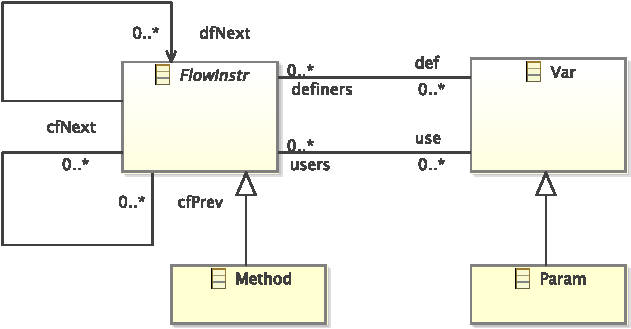
\includegraphics[width=0.6\linewidth]{../metamodel/DataFlowGraph}
  \caption{Metamodel classes related to data flow}
  \label{fig:data-flow-mm}
\end{figure}

\paragraph{Subtask 3.1.}
\label{sec:subtask-3.1}

For every local variable statement in the JaMoPP model, task 1's transformation
has to create a \verb|Var| object.  It's \verb|txt| attribute should be set to
the variable's name.  Similarly, a \verb|Param| object has to be created for
every method parameter.  Again, the \verb|txt| attribute should be set to the
parameter's name.

Furthermore, every flow instruction should be connected to the variables it
writes (the \verb|def| reference) and to the variables it reads (the \verb|use|
reference).  The method parameters are the \verb|def|-list of their method, the
statement \verb|a = b + c;| has a \verb|def| link to \verb|a|, and two
\verb|use| links to \verb|b| and \verb|c|, and the statement \verb|i++;| both
defines and uses \verb|i|.

Again, the result models of this subtask are contained in the \verb|results|
folder.  For every Java source file \verb|TestX|, there is a model
\verb|TestX-ControlFlowGraph-with-Vars.xmi| plus a PDF visualization of it.  In
case you've skipped this subtask, you can use them to tackle the next subtask.

\paragraph{Subtask 3.2.}
\label{sec:subtask-3.2}

The model resulting from applying the enhanced model-to-model transformation on
the JaMoPP syntax graphs followed by applying the control flow transformation
from task 2 to it is the source model for the data flow transformation to be
developed in this subtask.

It's sole purpose is to synthesize \verb|dfNext| links.  For every flow
instruction $n$, a \verb|dfNext| link has to be created from all nearest
control flow predecessors $m$ that define a variable which is used by $n$.  Or
formally:

\begin{align*}
  m \rightarrow_{dfNext} n  \iff {} & def(n) \cap use(m) \neq \emptyset\\
  ~\land {} & \exists~Path~m = n_0 \rightarrow_{cfNext} ... \rightarrow_{cfNext} n_k = n:\\
  & \left(def(n) \cap use(m)\right) \setminus \left(\bigcup_{0 < i < k}
    def(n_i)\right) \neq \emptyset
\end{align*}

That is, $n$ uses at least one variable defined by $m$, and there is a control
flow path from $m$ to $n$ in which at least one variable used by $n$ and
defined by $m$ is not redefined by intermediate flow instructions.

There are several ways to tackle this problem.  A simple one is to take the
definition literally, i.e., for every flow instruction search the nearest
control flow predecessors that define a variable used by instruction with
quadratic worst-case effort.  A more efficient and sophisticated algorithm is
described in the dragonbook \cite{Aho:CPTT}, chapter 9.1.  The models resulting
from this task which include control and data flow information are called
\emph{program dependence graphs} (PDG), and they play an important role in the
optimization phase in compilers \cite{Ferrante:1987:PDG:24039.24041}.

The method defined in \verb|Test0.java| is shown in
Listing~\ref{lst:java-ex-df}.  The program dependence graph that this subtasks
transformation has to generate is visualized in Figure~\ref{fig:pdg-test0} in
Appendix~\ref{sec:result-models}.

\begin{listing}
  \begin{minted}{java}
public int testMethod() {
    int a = 1;
    int b = 2;
    int c = a + b;
    a = c;
    b = a;
    c = a / b;
    b = a - b;
    return b * c;
}
  \end{minted}
  \caption{An example Java method for illustrating data flow
    (\texttt{Test0.java})}
  \label{lst:java-ex-df}
\end{listing}


The result models (including visualizations) are again available in the
\verb|results| directory.  They are named \verb|TestX-DataFlowGraph.{xmi,pdf}|.
Because the \verb|Var| objects were only needed for computing the data flow
links, they are deleted from the models in order to keep the visualizations
readable.

\subsection{Task 4: Validation}
\label{sec:task4-validation}

The fourth task is no strict transformation task.  Instead, the challenge is
validating the control flow graphs created by task 2, and the program
dependence graphs resulting from task 3.  Concretely, it should be checked if
all \verb|cfNext| and \verb|dfNext| links are set properly.

Since transformation experts have no time for testing their transformations in
the same way as programmers have no time to test their programs, it would be
fabulous if this boring work could be offloaded to other people.  Assume those
don't know anything about MDE in general or more specifically EMF (or whatever
modeling framework you are using), but they are great Java programmers who can
recite every section of the JLS \cite{Java7Spec} from the top of their heads.
So the task is to give them a simple tool that gets a program dependence graph
as input and all control and data flow links in an easy to write textual
syntax.  It should print all missing and all false links, i.e., all links
defined in the textual specification that don't occur in the model, and all
links occuring in the model that are not defined by the specification.

In the example Java programs provided in this case description project, every
statement and expressions occurs exactly once, e.g., there's is no method with
two \verb|i++;| statements.  As a result, for all PDGs generated from them, the
\verb|txt| attribute can be used to uniquely identify any object.  This will be
true for any additional methods that might be used for evaluation.

For example, such a specification for the method shown in
Listing~\ref{lst:java-ex-df} could be written like in
Listing~\ref{lst:example-validation}.

\begin{listing}
\begin{verbatim}
cfNext: "testMethod()"   --> "int a = 1;"
cfNext: "int a = 1;"     --> "int b = 2;"
cfNext: "int b = 2;"     --> "int c = a + b;"
cfNext: "int c = a + b;" --> "a = c;"
cfNext: "a = c;"         --> "b = a;"
cfNext: "b = a;"         --> "c = a / b;"
cfNext: "c = a / b;"     --> "b = a - b;"
cfNext: "b = a - b;"     --> "return b * c;"
cfNext: "return b * c;"  --> "Exit"

dfNext: "int a = 1;"     --> "int c = a + b;"
dfNext: "int b = 2;"     --> "int c = a + b;"
dfNext: "int c = a + b;" --> "a = c;"
dfNext: "a = c;"         --> "b = a;"
dfNext: "a = c;"         --> "c = a / b;"
dfNext: "a = c;"         --> "b = a - b;"
dfNext: "b = a;"         --> "c = a / b;"
dfNext: "b = a;"         --> "b = a - b;"
dfNext: "c = a / b;"     --> "return b * c;"
dfNext: "b = a - b;"     --> "return b * c;"
\end{verbatim}
  \caption{An example textual DSL for validating the program dependence graph
    of the method shown in Listing~\ref{lst:java-ex-df}}
  \label{lst:example-validation}
\end{listing}

There's no restrictions on the actual syntax except that it should be easy to
write for a Java programmer.


\section{Evaluation Criteria}
\label{sec:evaluation-criteria}

In the \verb|evaluation| directory, there is an OpenDocument spreadsheet
\verb|evaluation_sheet.ods| that will be used to score all submitted solutions.

Every voter should assign a score value in the range from 1 (not solved, or
very poor) to 5 (excellent) for each submitted solution and every task
separately.  For every solution, the average scores per tasks are weighted.
Task 1 is weighted with 30\%, Task 2 is weighted with 40\% because its
unquestionable the most complex one, and the tasks 3.1, 3.2, and 4 are weighted
with 10\% each.  So the typical model-to-model transformation tasks 1 and 3.1
have a weight of 40\% in total, the more graph transformation like tasks 2 and
3.2 have a total weight of 50\%, and the validation task 4 with its 10\% weight
might be the one that tipps the scales.

To score a task, voters should take into account the following criteria.  The
most important one is \emph{completeness \& correctness}, so it is weighted
with 50\%.  Another important factor weighted with 30\% is \emph{conciseness \&
  understandability}.  Lastly, the \emph{efficiency} of the solution is another
criterium that's weighted with the remaining 20\%.  To evaluate the latter,
further much larger Java methods and corresponding models for test-driving the
solutions will be provided.  Of course, those will use only the exactly same
Java language constructs as the existing examples.



\bibliography{ttc-2013-flowgraphs-case}
\bibliographystyle{alpha}

\appendix

\section{List of used JaMoPP Classifiers}
\label{sec:list-used-jamopp}

\begin{compactenum}
\item \verb|classifiers.Class|
\item \verb|containers.CompilationUnit|
\item \verb|expressions.AdditiveExpression|
\item \verb|expressions.AssignmentExpression|
\item \verb|expressions.EqualityExpression|
\item \verb|expressions.MultiplicativeExpression|
\item \verb|expressions.RelationExpression|
\item \verb|expressions.SuffixUnaryModificationExpression|
\item \verb|literals.DecimalIntegerLiteral|
\item \verb|members.ClassMethod|
\item \verb|modifiers.Public|
\item \verb|modifiers.Static|
\item \verb|operators.Addition|
\item \verb|operators.Assignment|
\item \verb|operators.Division|
\item \verb|operators.Equal|
\item \verb|operators.GreaterThan|
\item \verb|operators.LessThan|
\item \verb|operators.MinusMinus|
\item \verb|operators.Multiplication|
\item \verb|operators.PlusPlus|
\item \verb|operators.Subtraction|
\item \verb|parameters.OrdinaryParameter|
\item \verb|references.IdentifierReference|
\item \verb|statements.Block|
\item \verb|statements.Break|
\item \verb|statements.Condition|
\item \verb|statements.Continue|
\item \verb|statements.ExpressionStatement|
\item \verb|statements.JumpLabel|
\item \verb|statements.LocalVariableStatement|
\item \verb|statements.Return|
\item \verb|statements.WhileLoop|
\item \verb|types.ClassifierReference|
\item \verb|types.Int|
\item \verb|types.Void|
\item \verb|variables.LocalVariable|
\end{compactenum}

\clearpage
\section{Example Result Models}
\label{sec:result-models}

\begin{figure}[h!]
  \centering
  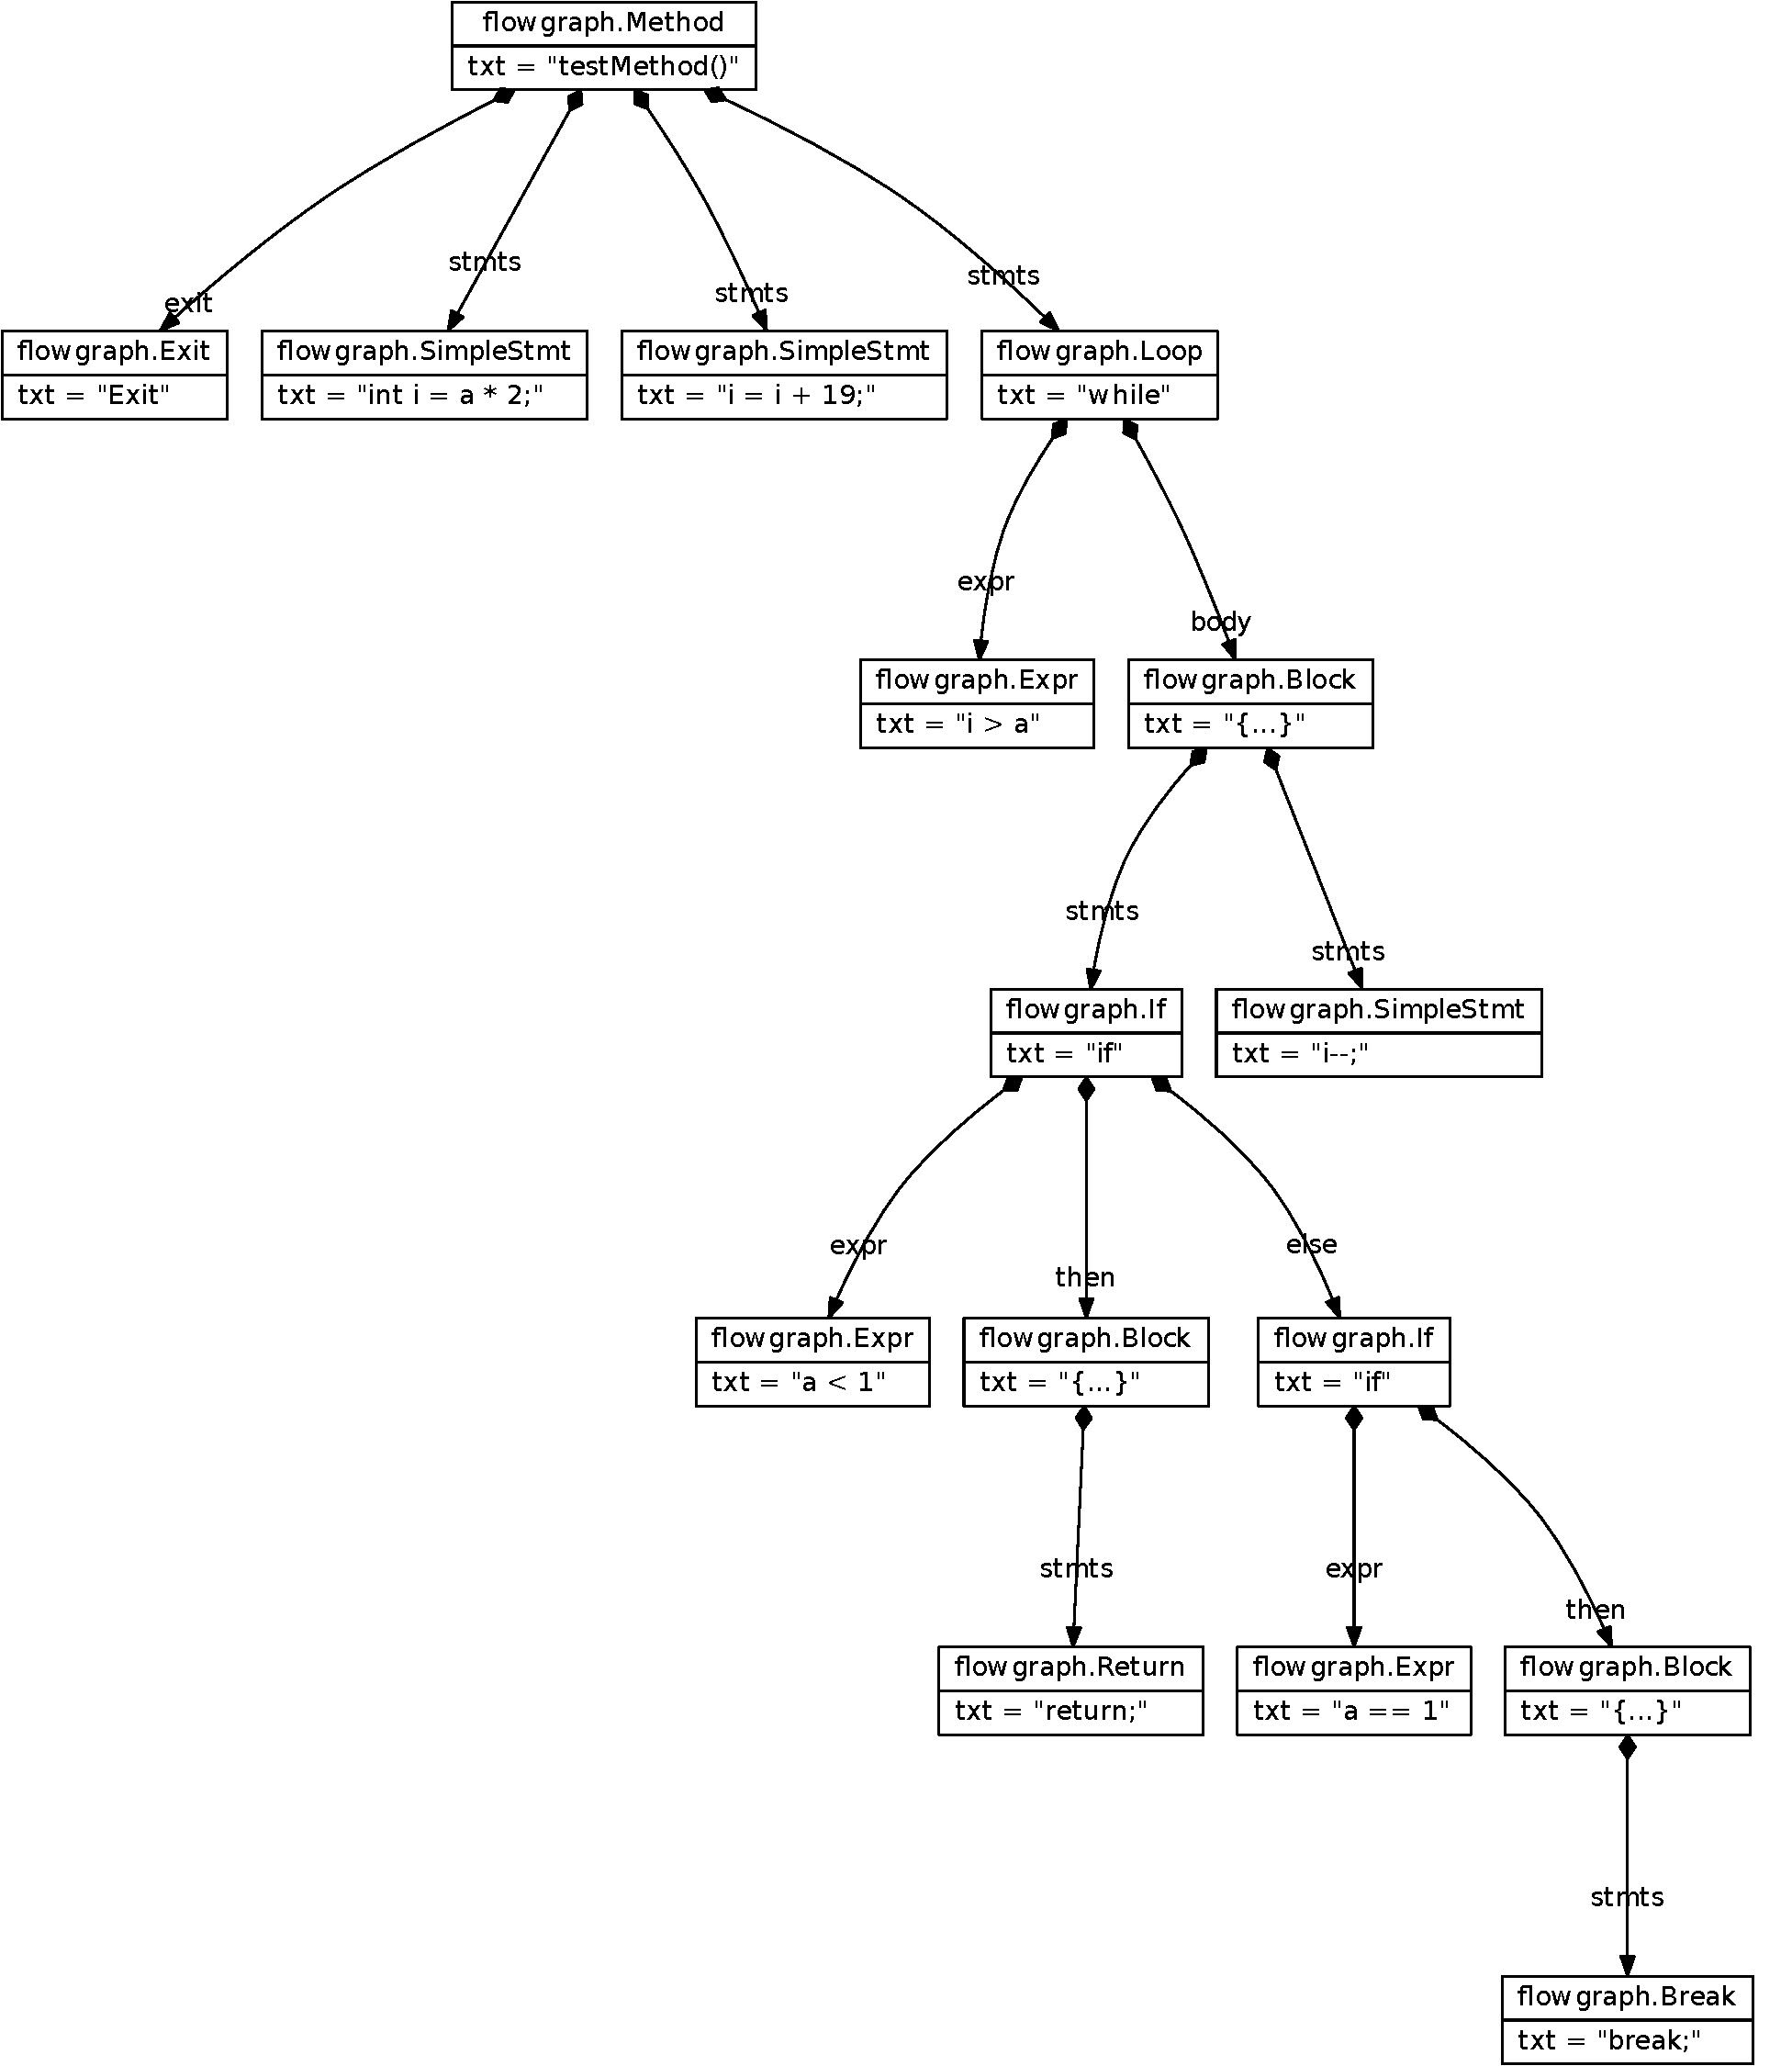
\includegraphics[width=\linewidth]{../results/Test1-StructureGraph}
  \caption{Structure graph corresponding to \texttt{Test1.java}}
  \label{fig:sg-test1}
\end{figure}

\begin{figure}[h!]
  \centering
  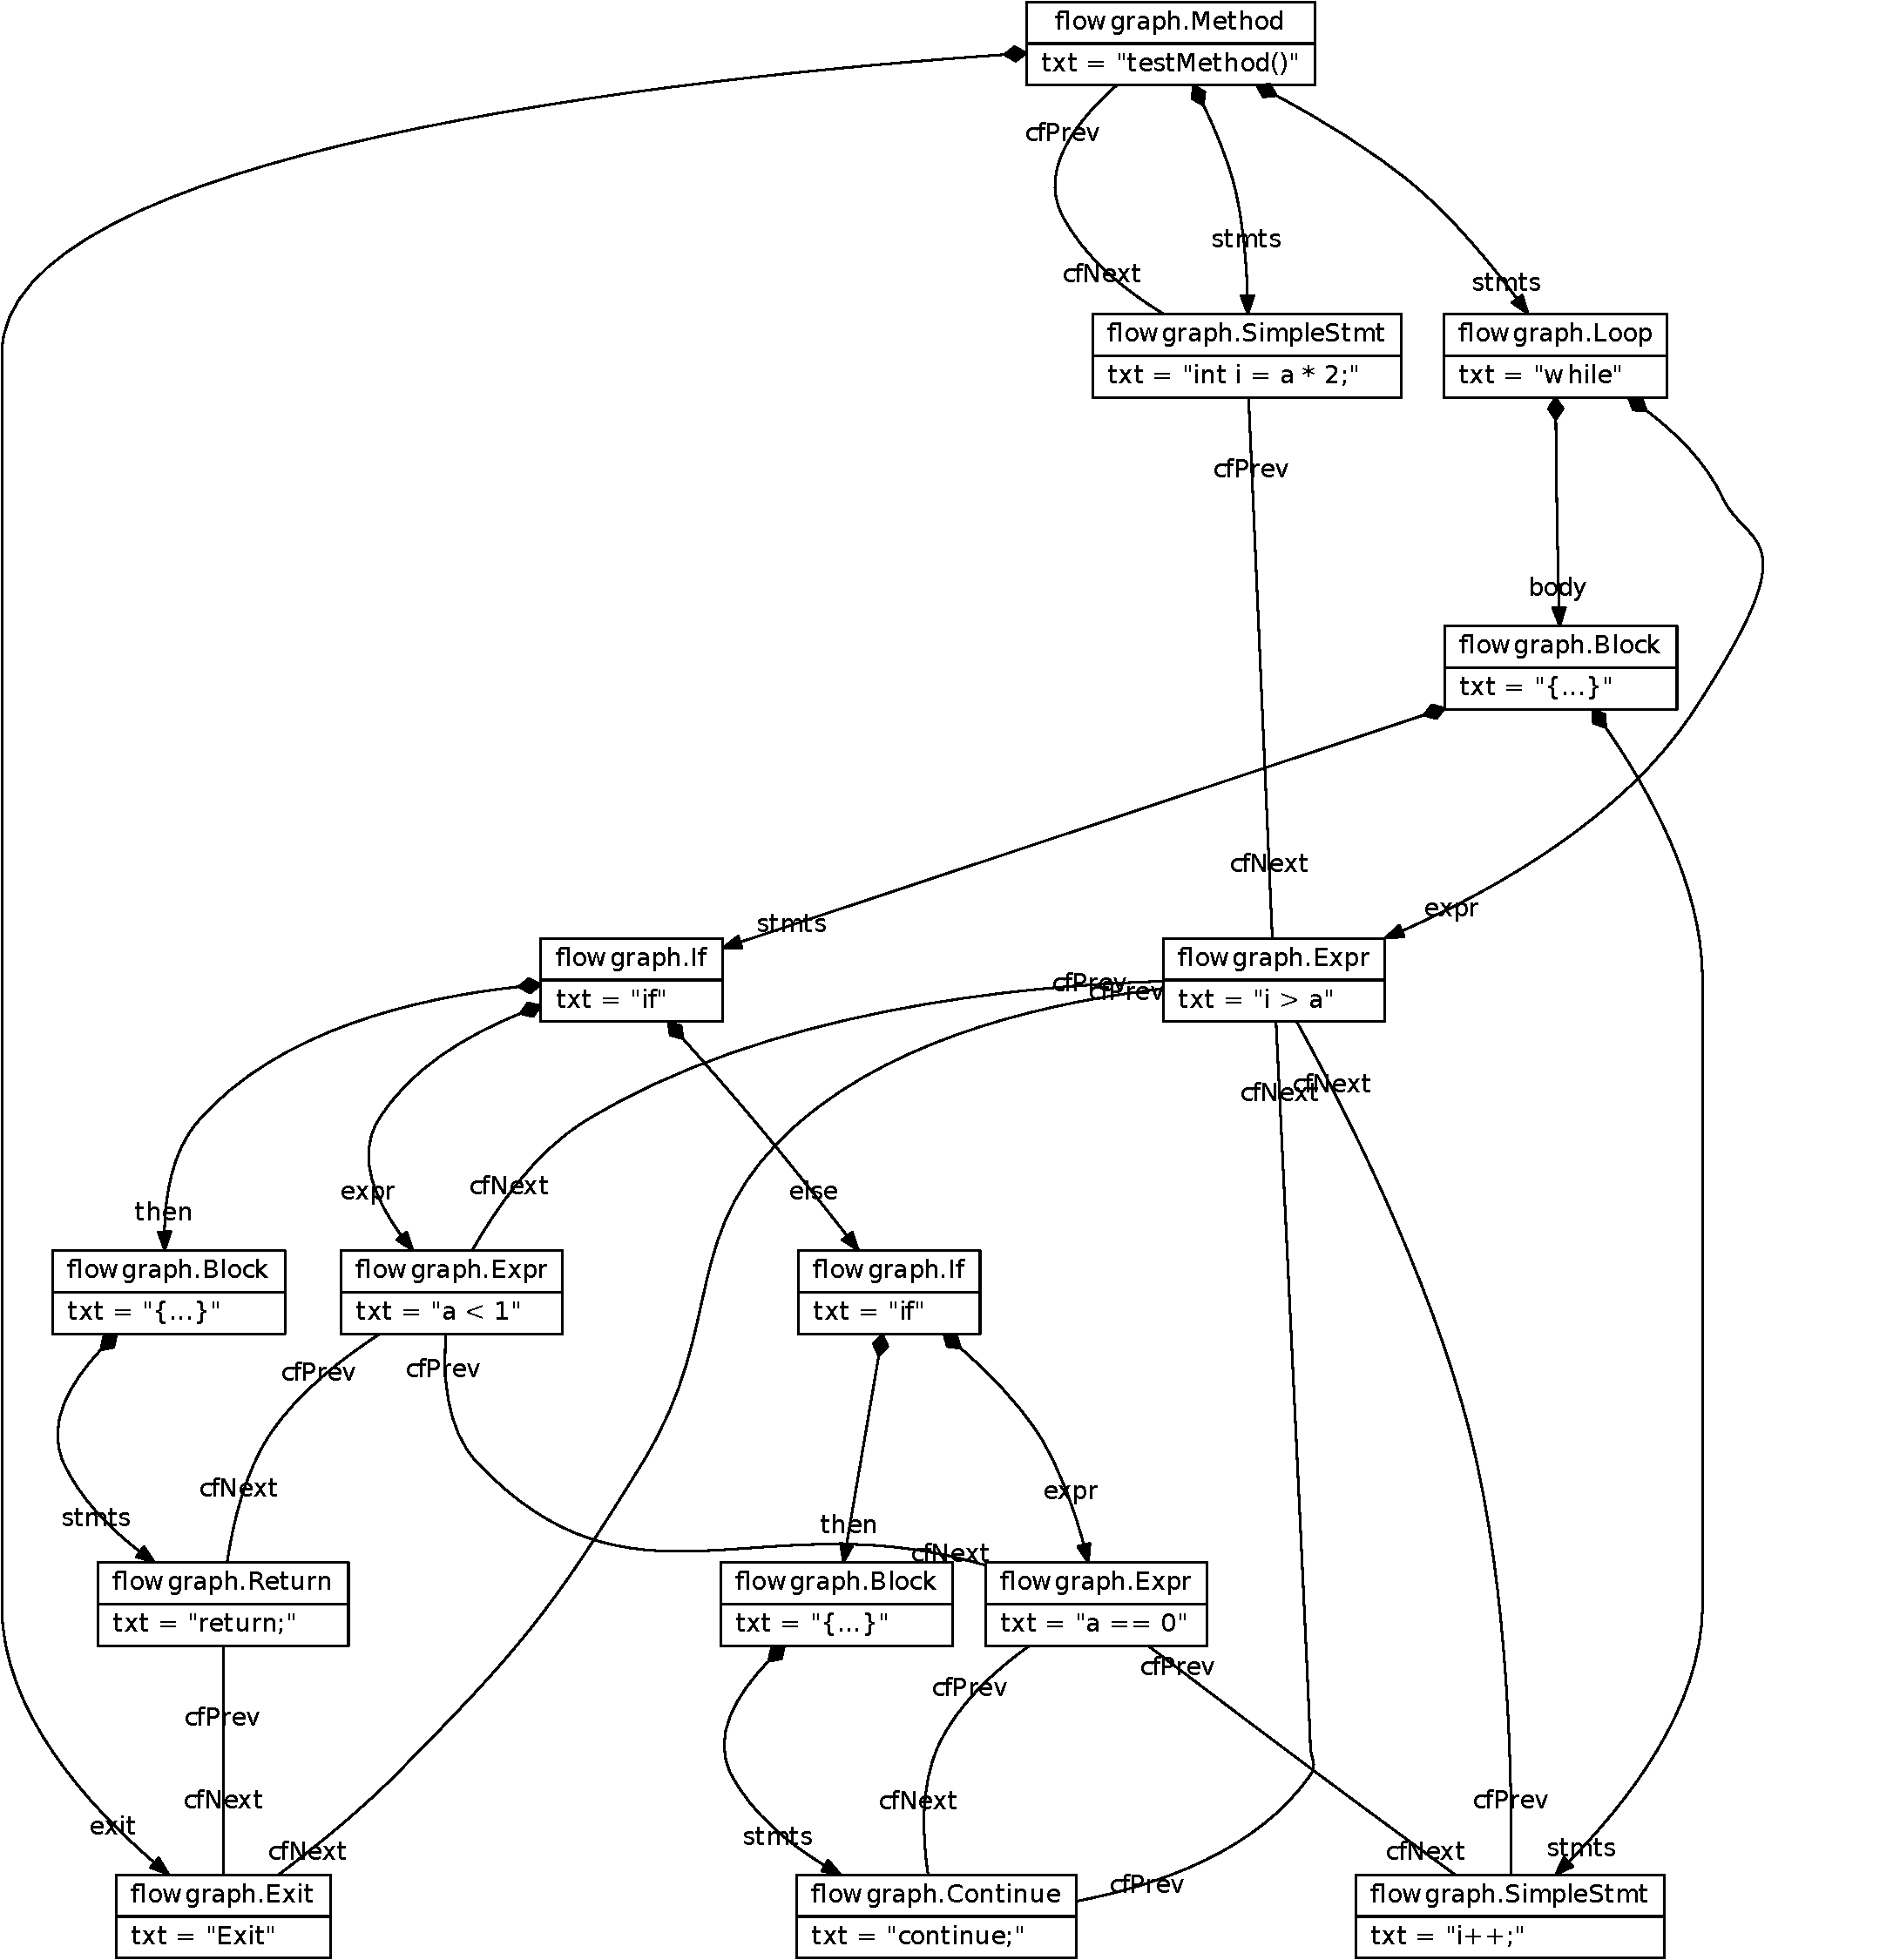
\includegraphics[width=\linewidth]{../results/Test2-ControlFlowGraph}
  \caption{Control flow graph corresponding to \texttt{Test2.java}}
  \label{fig:cfg-test2}
\end{figure}

\begin{figure}[h!]
  \centering
  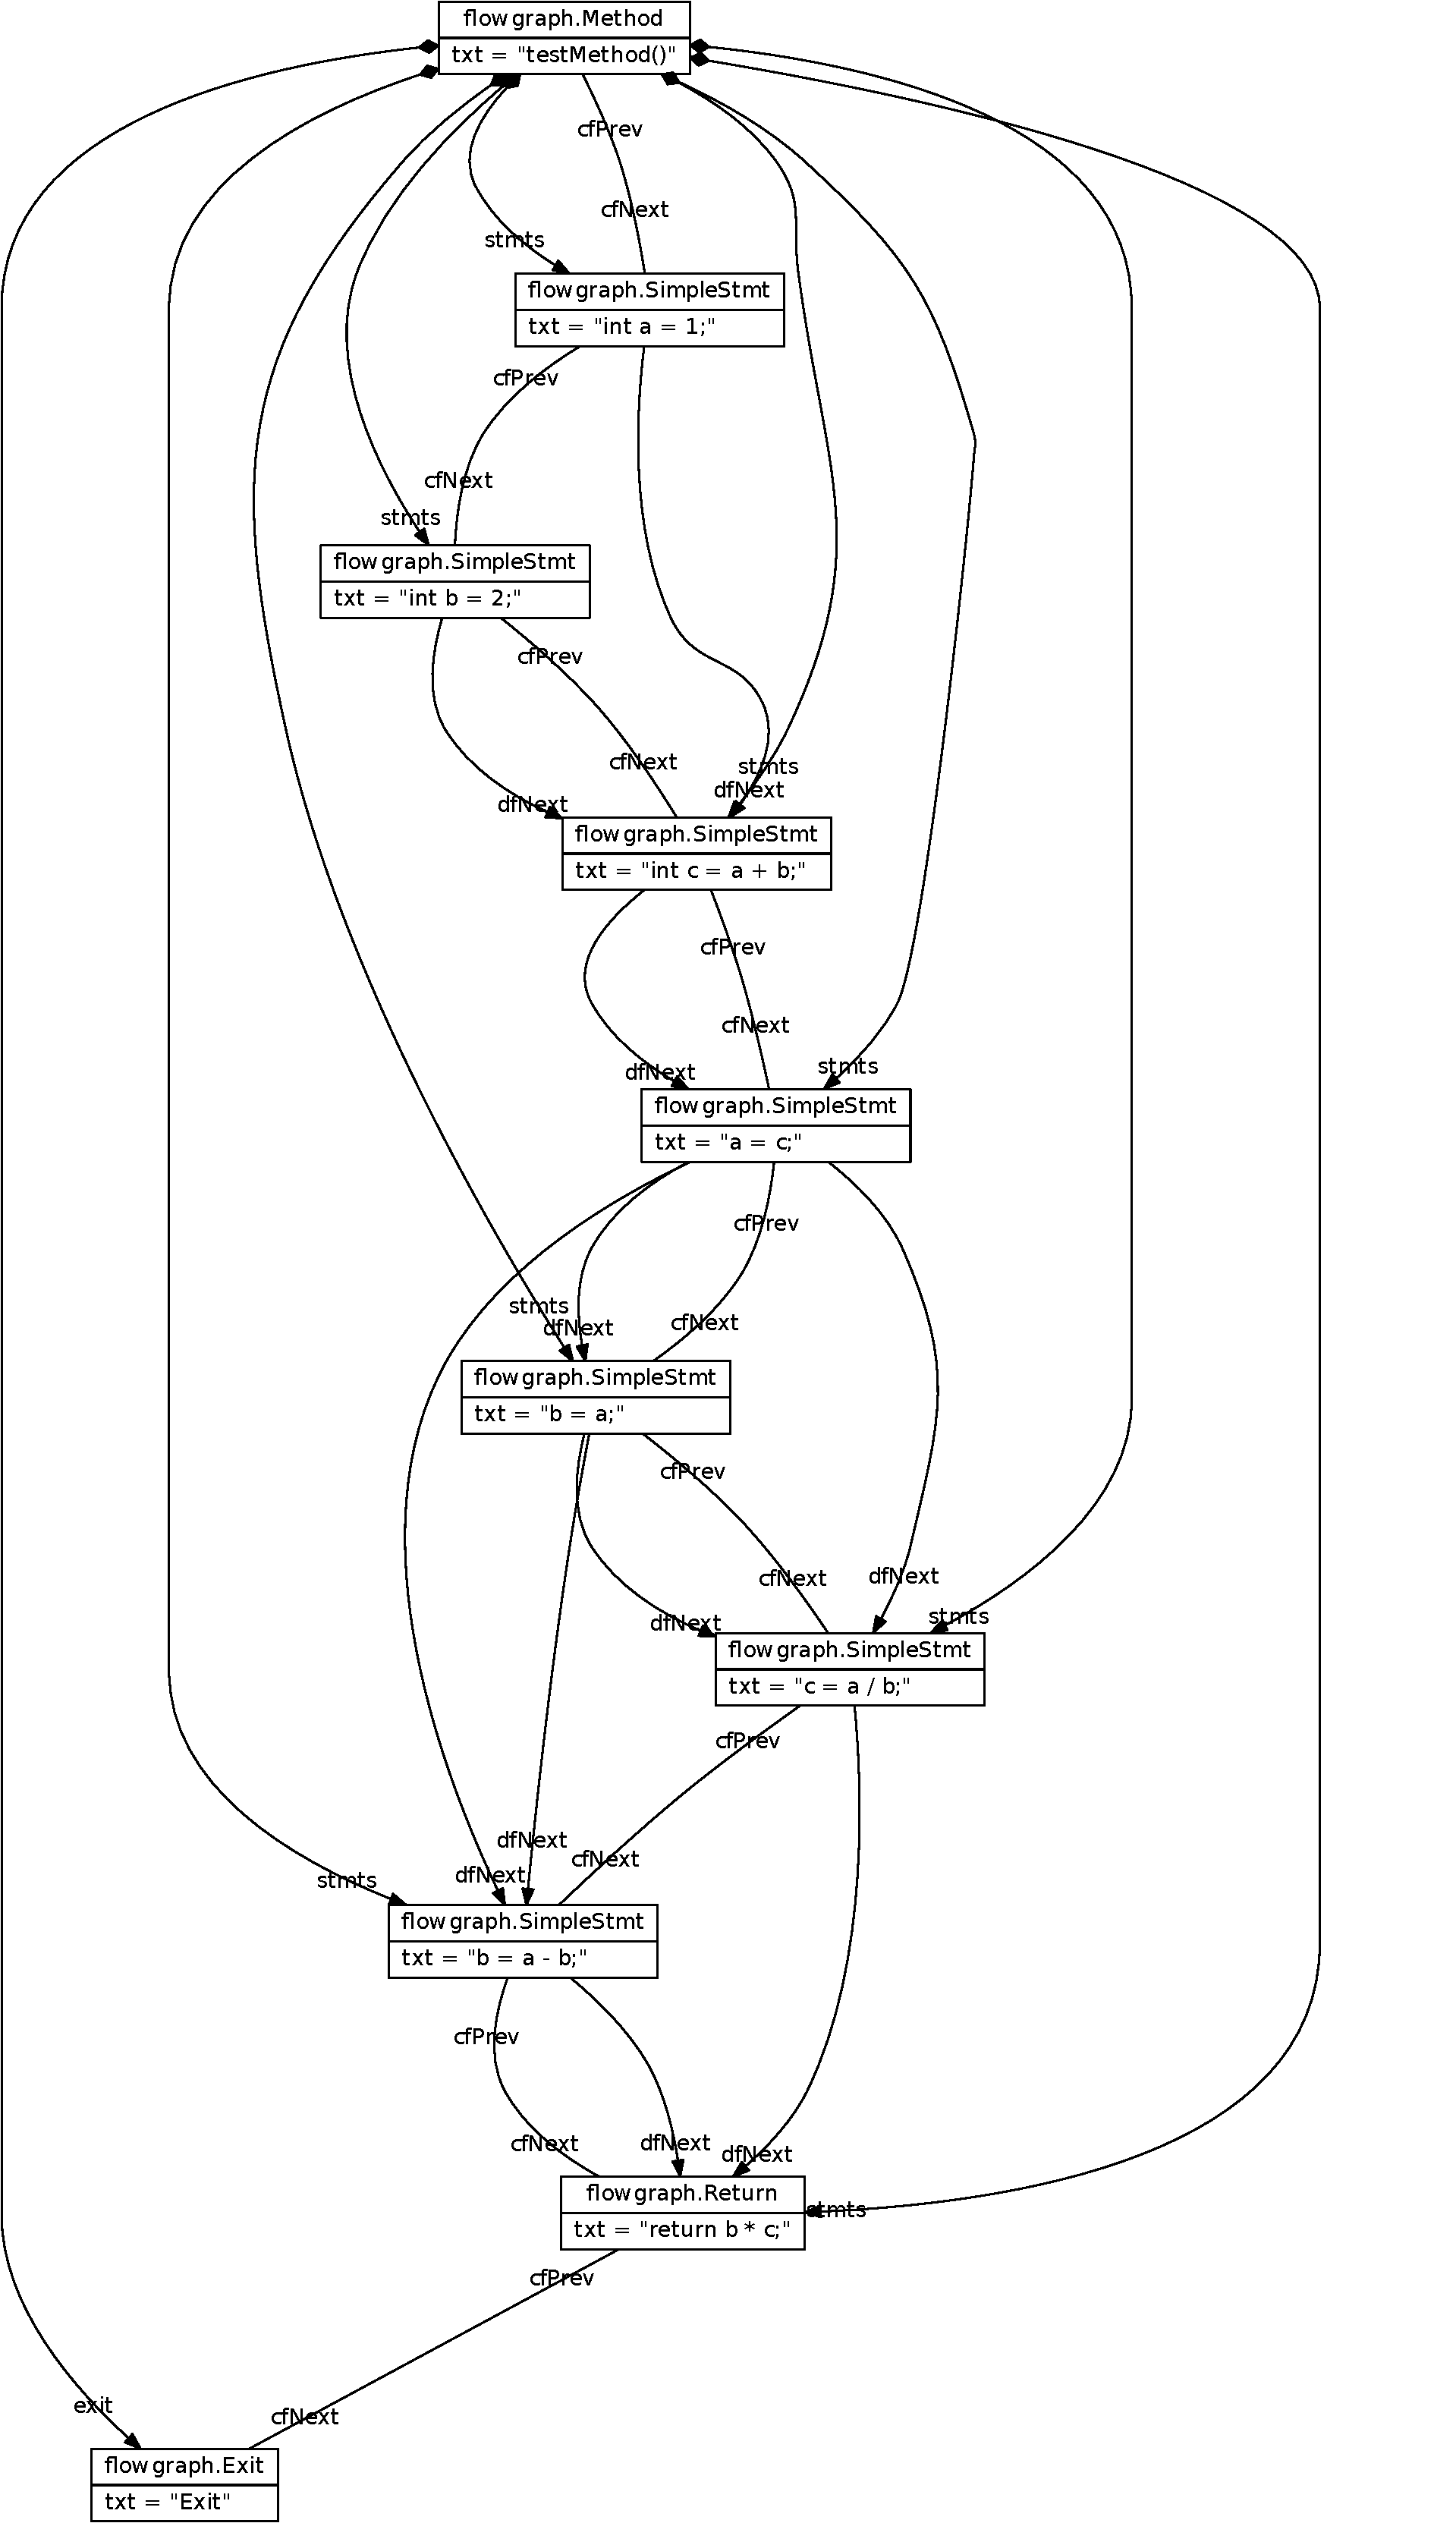
\includegraphics[height=0.9\textheight]{../results/Test0-DataFlowGraph}
  \caption{Program dependence graph corresponding to \texttt{Test0.java}}
  \label{fig:pdg-test0}
\end{figure}

\end{document}

%%% Local Variables:
%%% mode: LaTeX
%%% TeX-master: t
%%% fill-column: 79
%%% TeX-engine: xetex
%%% TeX-engine-alist: ((xetex "XeTeX" "xetex -shell-escape -output-driver='xdvipdfmx -V 5'" "xelatex -shell-escape -output-driver='xdvipdfmx -V 5'" "xetex"))
%%% End:
